\section{Neurale Netwerken}

\subsection{Niet-lineaire \textit{decision boundary}}

We kunnen ook niet-lineaire \textit{decision boundaries} hebben. Dit doen we door hogere orde-modellen te bouwen. Zo kunnen we bijvoorbeeld wanneer we een $x_{1}$ en een $x_{2}$ hebben, een $x_{3}$, $x_{4}$ en $x_{5}$ toevoegen die respectievelijk gelijk zijn aan $x_{1}^{2}$, $x_{2}^{2}$ en $x_{1}^{2} x_{2}^{2}$. Het aantal parameters kan berekend worden als:

\begin{equation}
	{d + n \choose d} = \frac{(d+n)!}{d! n!}
	\label{eq:nr-of-parameters}
\end{equation}
\noindent
waarbij $d$ de \textit{degree} van het model is en $n$ het aantal \textit{features}. Voor bovenstaand geval is dit dus: 
\begin{equation*}
	{2 + 2 \choose 2} = \frac{4!}{2! 2!} = \frac{\ldots4\cdot 3\cdot 2\cdot 1}{2\cdot 1\cdot 2\cdot 1} = 6
\end{equation*}
\newpage
\noindent
We zullen inderdaad 6 parameters hebben, namelijk 5 gewichten en de \textit{bias}. We kunnen echter wel direct aan formule \ref{eq:nr-of-parameters} zien dat dit heel slecht zal schalen met het aantal \textit{features}. We zullen dus op zoek moeten gaan naar een manier om met minder complexiteit een goed model te vinden. \\
\newline
Figuur \ref{fig:non-linear-classification} toont een voorbeeld van een ongerelateerd niet-lineair classificatieprobleem ter illustratie.
\begin{figure}[h]
	\centering
	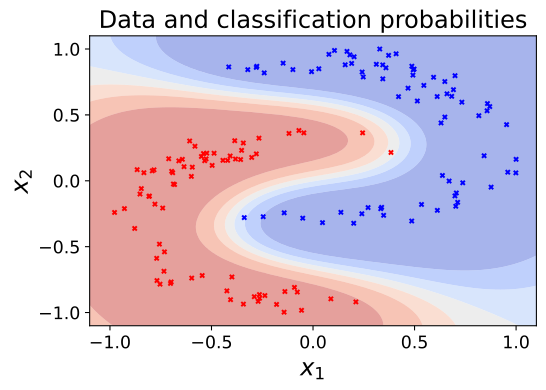
\includegraphics[width=0.3\textwidth]{images/12-non-linear-classification.png}
	\caption{Voorbeeld van niet-lineaire classificatie}
	\label{fig:non-linear-classification}
\end{figure}

\subsection{Modelvoorstelling bij neurale netwerken}

Zoals we eerder al gezien hebben is logistische regressie eigenlijk een neuraal netwerk met één node. Figuur \ref{fig:neural-network-model-log-reg} stelt dit grafisch voor. 

\begin{figure}[h]
	\centering
	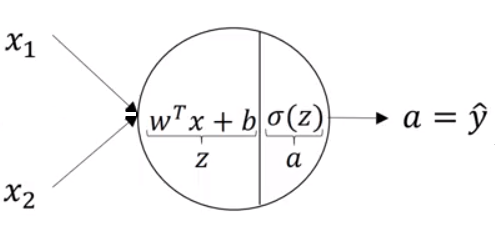
\includegraphics[width=0.4\textwidth]{images/13-neural-network-model-log-reg.png}
	\caption{Logistische regressie als neuraal netwerk}
	\label{fig:neural-network-model-log-reg}
\end{figure}
\noindent
De uitgang $a$ wordt ook wel de activatie genoemd. $z$ wordt ook wel logit genoemd. We kunnen dit blokje van Figuur \ref{fig:neural-network-model-log-reg} nu herhaaldelijk gaan gebruiken om het model van Figuur \ref{fig:neural-network-model-1} te bekomen. 

\begin{figure}[h]
	\centering
	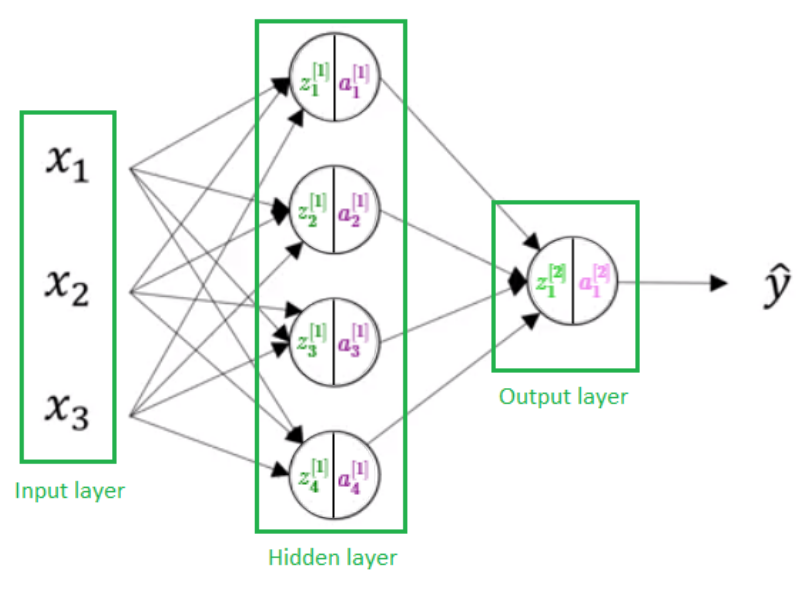
\includegraphics[width=0.5\textwidth]{images/14-neural-network-model-1.png}
	\caption{Neuraal netwerk met 1 \textit{hidden layer}}
	\label{fig:neural-network-model-1}
\end{figure}

\noindent
We kunnen de logit en activatie van elke node berekenen. Dit doen we als volgt:
\begin{equation}
	z_{i}^{[j]} = \vec{w}_{i}^{[j]} \cdot \vec{x} + b_{i}^{[j]}
\end{equation}
\begin{equation}
	a_{i}^{[j]} = \sigma(z_{i}^{[j]})
\end{equation}
\noindent
Hierbij wijst $j$ op de laag van de node en $i$ op de node binnen die laag $j$. We kunnen deze berekening voor $z_{i}^{[j]}$ natuurlijk ook algebraïsch voorstellen als:
\begin{equation}
	z_{i}^{[j]} = \vec{w}_{i}^{[j]^{T}} \vec{x} + b_{i}^{[j]}
\end{equation}
\noindent
Voor de tweede node van laag 1 (de \textit{hidden layer} van Figuur \ref{fig:neural-network-model-1}), is deze berekening gelijk aan:
\begin{equation*}
	z_{2}^{[1]} = \vec{w}_{2}^{[1]} \cdot \vec{x} + b_{2}^{[1]}
\end{equation*}
\begin{equation*}
	a_{2}^{[1]} = \sigma(z_{2}^{[1]})
\end{equation*}
We kunnen ook een formule opstellen om direct de hele laag te berekenen:
\begin{equation}
	\vec{z}^{[j]} = W^{[j]} \cdot \vec{x} + \vec{b}^{[j]}
\end{equation}
\begin{equation}
	\vec{a}^{[j]} = \sigma(\vec{z}^{[j]})
\end{equation}
\noindent
Voor het model van Figuur \ref{fig:neural-network-model-1} levert dit de volgende vergelijkingen op, met telkens de dimensie van de vector er bij vermeld ter verduidelijking:
\begin{equation*}
	\underset{4\times1}{\vec{z}^{[1]}} = \underset{4\times3}{W^{[1]}} \cdot \underset{3\times1}{\vec{x}} + \underset{4\times1}{\vec{b}^{[1]}}
\end{equation*}
\begin{equation*}
	\underset{4\times1}{\vec{a}^{[1]}} = \underset{4\times1}{\sigma(\vec{z}^{[1]})}
\end{equation*}
\begin{equation*}
	\underset{1\times1}{\vec{z}^{[2]}} = \underset{1\times4}{W^{[2]}} \cdot \underset{4\times1}{\vec{a}^{[1]}} + \underset{1\times1}{\vec{b}^{[2]}}
\end{equation*}
\begin{equation*}
	\underset{1\times1}{\vec{a}^{[2]}} = \underset{1\times1}{\sigma(\vec{z}^{[2]}) }
\end{equation*}
\noindent
Dit model kan uitgebreid worden tot meerdere lagen met een verschillend aantal knopen per laag, zoals op Figuir \ref{fig:neural-network-model-2}.
\begin{figure}[h]
	\centering
	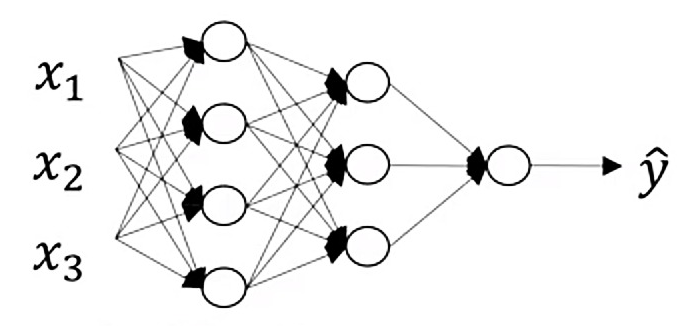
\includegraphics[width=0.5\textwidth]{images/15-neural-network-model-2.png}
	\caption{Neuraal netwerk met 2 \textit{hidden layers}}
	\label{fig:neural-network-model-2}
\end{figure}

\paragraph{Neurale netwerken in Python}

We kunnen gebruik maken van Tensorflow en Keras om een neuraal netwerk te implementeren in Python. Als we het model van Figuur \ref{fig:neural-network-model-2} zouden willen implementeren, ziet dat er als volgt uit:
\begin{lstlisting}
	model = Sequential(
	    [
	        tf.keras.Input(shape=(3,)), 
	        Dense(4, activation='sigmoid'),
	        Dense(3, activation='sigmoid'),
	        Dense(1, activation='sigmoid'),
	    ], name = "my_model"
	)
\end{lstlisting}
\begin{lstlisting}
	# Examine Weights shapes
	[layer1, layer2, layer3] = model.layers
	W1,b1 = layer1.get_weights()
	W2,b2 = layer2.get_weights()
	W3,b3 = layer3.get_weights()
	print(f"W1 shape = {W1.shape}, b1 shape = {b1.shape}") 
	# Output: W1 shape = (3, 4), b1 shape = (4,)
	print(f"W2 shape = {W2.shape}, b2 shape = {b2.shape}") 
	# Output: W2 shape = (4, 3), b2 shape = (3,)
	print(f"W3 shape = {W3.shape}, b3 shape = {b3.shape}") 
	# Output: W3 shape = (3, 1), b3 shape = (1,)
\end{lstlisting}

\subsection{\textit{Gradient descent} bij neurale netwerken}

Aangezien neurale netwerken zoals we ze nu zien een combinatie is van ons logistische regressie-model, zal de kostfunctie en \textit{gradient descent} identiek werken, met enkel een toename van de parameters. Voor het voorbeeld van Figuur \ref{fig:neural-network-model-1} hebben we de volgende parameters: $W^{[1]}$, $b^{[1]}$, $W^{[2]}$ en $b^{[2]}$. Deze hebben respectievelijk de dimensies $n^{[1]}\times n^{[0]}$, $n^{[1]}\times 1$, $n^{[2]}\times n^{[1]}$ en $n^{[2]}\times 1$ waarbij $n^{[0]}$, $n^{[1]}$ en $n^{[2]}$ respectievelijk staan voor het aantal input \textit{features}, het aantal nodes van laag 1 en het aantal nodes van laag 2. De kostfunctie is gelijk aan $J(W^{[1]}, b^{[1]}, W^{[2]}, b^{[2]}) = \frac{1}{m} \sum_{i=1}^{m} L(\hat{y}^{(i)}, y^{(i)})$ waarbij $\hat{y}^{(i)}$ de predictie en $y^{(i)}$ het label is. De predictie komt overeen met de activatie van het model. \\
\newline
We gaan niet te diep in op \textit{gradient descent}. Bij \textit{forward propagation} gaan we van ingang naar uitgang en zullen we dus de kostfunctie berekenen. Bij \textit{backpropagation} gaan we in de omgekeerde richting werken en berekenen we de partiële afgeleiden van de kostfunctie naar $W$ en $b$ en passen we hun waarden op basis hiervan aan. Dit zullen we opnieuw herhaaldelijk uitvoeren tot we convergentie bereiken. 

\paragraph{\textit{Gradient descent} in Python}
Nadat we ons model geïmplementeerd hebben, kunnen we een kostfunctie opstellen voor het model en \textit{gradient descent } toepassen. Dit doen we als volgt:

\begin{lstlisting}
	model.compile(
	    loss=tf.keras.losses.BinaryCrossentropy(),
	    optimizer=tf.keras.optimizers.Adam(0.001),
	)
\end{lstlisting}

\paragraph{Predictie in Python}
Hierna kunnen we ons model trainen en het vervolgens gebruiken om een voorspelling voor bijvoorbeeld het eerste element van onze input te maken. Hiervoor kunnen we de volgende code gebruiken:

\begin{lstlisting}
	# Het model trainen
	model.fit(
	    X,y,
	    epochs=20
	)
	# Een voorspelling maken
	prediction = model.predict(X[0])
	if prediction >= 0.5:
	    yhat = 1
	else:
	    yhat = 0
\end{lstlisting}
\noindent
Het aantal epochs geeft aan hoe vaak de dataset gebruikt moet worden tijdens het trainen. Om efficiënt te werken wordt de dataset in Tensorflow gesplitst in batches van 32. Deze parameter zouden we ook kunnen aanpassen in `\textit{model.fit()}'.

\subsection{\textit{Multi-class} classificatie}

Tot nu toe hebben we enkel binaire classificatie besproken waarbij we 2 klassen hebben, namelijk 0 en 1. We kunnen echter ook \textit{multi-class} classificatie hebben waarbij er meer dan 2 output-klassen zijn. Het voornaamste verschil zit er hier in dat we in ons model in de output-laag niet één knoop hebben, maar evenveel knopen als het aantal klassen dat we hebben.

\subsection{Kostfunctie voor \textit{multi-class} classificatie}

We kunnen nu ook de kostfunctie gaan uitbreiden voor \textit{multi-class} classificatie. Als $K$ het aantal klassen is, bekomen we voor de \textit{loss}-functie:

\begin{equation}
	L = - \frac{1}{m} \sum_{k=1}^{K} y_{k} ln( \hat{y}_{k})
\end{equation}
\noindent
Dit levert ons de volgende kostfunctie op:
\begin{equation}
	J(W^{[1]}, b^{[1]}, \ldots , W^{[L]}, b^{[L]}) = - \frac{1}{m} \sum_{i=1}^{m} \sum_{k=1}^{K} y_{k}^{(i)} ln( \hat{y}_{k}^{(i)})
\end{equation}

\subsection{Softmax}
\label{ch:softmax}
Tot nu toe hebben we altijd gekeken naar een \textit{cross entropy loss}. Er bestaat echter ook een andere optie: softmax. Hierbij gaan we de uitgang van onze classificatie normaliseren zodat de som van de probabiliteiten voor de verschillende klassen gelijk is aan 1. Het voordeel hiervan is dat we direct kunnen zien wat de kans is dat ons resultaat tot een bepaalde klasse behoort.\\
\newline
Dit doen we door, nadat we $\vec{z}^{[L]}$ berekend hebben, eerst $\vec{t}$ te berekenen, waarbij $t_{i}$ gelijk is aan:
\begin{equation}
	t_{i} = e^{z_{i}^{[L]}}
\end{equation}
\noindent
Vervolgens kunnen we onze activatie $\vec{a}^{[L]}$ berekenen waarbij $a_{i}^{[L]}$ gelijk is aan:
\begin{equation}
	a_{i}^{[L]} = \frac{t_{i}}{\sum_{i=1}^{K} t_{i}}
\end{equation}
\noindent
De \textit{loss} - en kostfunctie zal hetzelfde blijven, alleen zal $\hat{y}$ nu op een andere manier berekend worden. 

\paragraph{Softmax in Python}

We kunnen de softmax functie als volgt in Python implementeren (al is er ook een ingebouwd softmax-functie in Tensorflow):

\begin{lstlisting}
	def my_softmax(z): # Identiek aan tf.nn.softmax(z)
	    """ Softmax converts a vector of values to a probability distribution.
	    Args:
	        z (ndarray (N,))  : input data, N features
	    Returns:
	        a (ndarray (N,))  : softmax of z
	    """
	    N = len(z)
	    a = np.zeros(N)
	    ez_sum = 0
	    for k in range(N):                
	        ez_sum += np.exp(z[k])       
	    for j in range(N):                
	        a[j] = np.exp(z[j])/ez_sum   
	    return a
\end{lstlisting}

\subsection{Activatiefuncties}

\subsubsection{Activatiefuncties}

Tot nu toe hebben we altijd gewerkt met een vaste activatiefunctie. We zouden echter ook kunnen werken met een activatiefunctie per laag. Dit zullen we dan voorstellen als $\vec{a}^{[i]} = \sigma^{[i]}(\vec{z}^{[i]})$ waarbij $i$ gaat van 1 tot $L$. \\
\newline
Typisch zullen we in onze verborgen laag gebruik maken van een RELU activatiefunctie en in onze output laag van de logistische functie (sigmoid) of softmax. We zullen de verschillende activatiefuncties nog eens kort even bespreken.

\paragraph{Sigmoid}

De sigmoid hebben we al eerder besproken in deel \ref{ch:logistic-regression} van deze samenvatting. Hij wordt beschreven door formule \ref{eq:sigmoid} (al zullen we nu het symbool $a$ gebruiken in plaats van $g$) en het verloop ziet er uit zoals op Figuur \ref{fig:sigmoid}. \\
\newline
De sigmoid wordt typisch gebruikt aan de output laag. We stellen vast dat als we deze functie afleiden naar $z$, dat we het volgende bekomen:
\begin{equation}
	\frac{da}{dz} = a (1 - a)
\end{equation}
\noindent
We kunnen ook afleiden dat deze afgeleide ongeveer gelijk zal zijn aan 0 voor zeer grote en kleine waarden van $z$. 

\paragraph{RELU}

RELU staat voor \textit{rectified linear unit} en wordt typisch gebruikt in de verborgen lagen. De RELU functie wordt voorgesteld door de volgende vergelijking:
\begin{equation}
	a(z) = \max(0, z)
\end{equation}
\noindent
Dit levert de volgende afgeleide op:
\begin{equation}
	\frac{da}{dz} = 1
\end{equation}
\noindent
Het voordeel hiervan is dat wanneer we \textit{backpropagation} toepassen, we veel sneller zullen convergeren in vergelijking met de sigmoid functie die een zeer kleine waarde heeft voor zijn afgeleide voor kleine en grote waarden van $z$. Deze afgeleide is namelijk een onderdeel van de partiële afgeleide van de kostfunctie. \\
\newline
De grafiek van de RELU functie ziet er uit zoals op Figuur \ref{fig:relu}.
\begin{figure}[h]
	\centering
	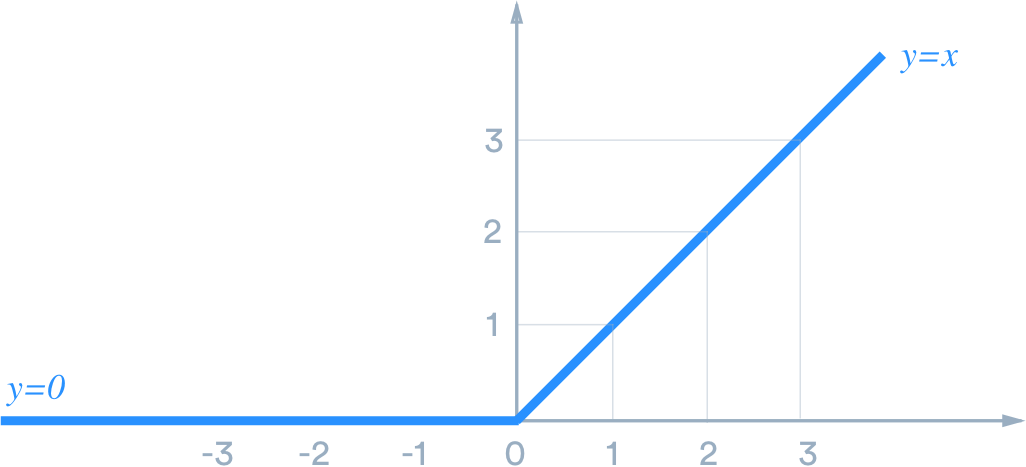
\includegraphics[width=0.5\textwidth]{images/16-relu.png}
	\caption{RELU functie}
	\label{fig:relu}
\end{figure}
\newpage
\paragraph{Leaky RELU}

De Leaky RELU functie is een variant van de RELU functie. In plaats van het maximum te nemen van 0 en $z$, wordt er hier het maximum genomen van het product van $z$ met een constante en $z$. Dit levert volgende vergelijking en de grafiek van Figuur \ref{fig:leaky-relu} op:
\begin{equation}
	a(z) = \max(cz, z)
\end{equation}

\begin{figure}[h]
	\centering
	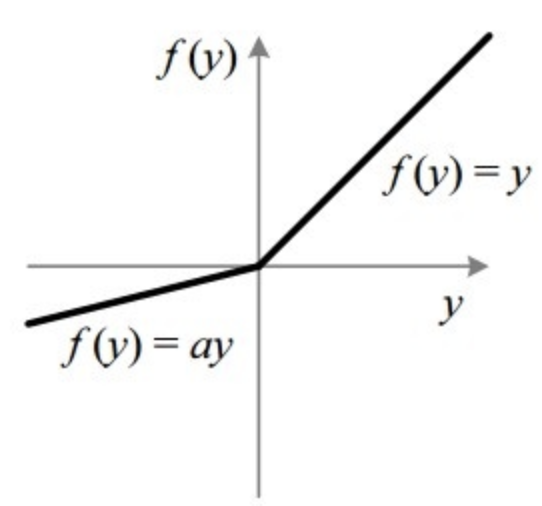
\includegraphics[width=0.25\textwidth]{images/17-leaky-relu.png}
	\caption{Leaky RELU functie}
	\label{fig:leaky-relu}
\end{figure}
\noindent
Aangezien deze activatiefunctie niet heel interessant is, zullen we deze verder ook niet bespreken.

\paragraph{Softmax}

Softmax is zonet uitgebreid besproken in sectie \ref{ch:softmax}. Dit zullen we hier dus niet opnieuw doen.

\paragraph{Activatiefuncties in Python}
We voegen de activatiefunctie toe aan onze laag wanneer we ons model implementeren. Hieronder zijn de verschillende activatiefuncties die we gezien hebben terug te vinden zoals we ze in Python gebruiken:

\begin{lstlisting}
	# Geen activatie
  Dense(25, activation='linear')
	# Sigmoid activatie
	Dense(25, activation='sigmoid')
	# RELU activatie
	Dense(25, activation='relu')
	# Softmax activatie
	Dense(25, activation='softmax')
\end{lstlisting}
\noindent
Het zal echter numeriek stabieler zijn wanneer we softmax niet in de output laag van ons model steken, maar groeperen met onze kostfunctie. Om dit te doen, zullen we lineaire activatie gebruiken in de laatste \textit{Dense} laag van onze model en wanneer we ons model compileren, `\textit{from\_logits=True}' toevoegen aan onze \textit{loss}:
\begin{lstlisting}
	model = Sequential(
	    [
	        tf.keras.Input(shape=(400,)),     
	        Dense(25, activation='relu', name = "layer1"),
	        Dense(15, activation='relu',  name = "layer2"),   
	        Dense(10, activation='linear', name = "layer3"),  
	    ], name = "my_model"
	)
	model.compile(loss=tf.keras.losses.SparseCategoricalCrossentropy(from_logits=True))
\end{lstlisting}
\noindent
Dit zal er wel voor zorgen dat onze output geen kansen zijn. Als we dit wel willen, zullen we de softmax functie nog moeten toepassen.

\subsubsection{Activatiefuncties bij regressieprobleem}

De vorige activatiefuncties zijn allemaal niet-lineair en worden gebruikt bij classificatieproblemen. Wanneer we een regressieprobleem hebben, zullen we geen extra niet-lineaire activatiefunctie toevoegen, maar $\vec{a}^{[L]}$ direct gelijkstellen aan $\vec{z}^{[L]}$. We kunnen neurale netwerken dus ook gebruiken om regressieproblemen op te lossen. 

\subsubsection{Doel van niet-lineaire activatiefuncties}

We hebben de niet-lineariteit van onze activatiefunctie nodig om de complexiteit van ons model te gebruiken. Als we de niet-lineariteit er uit halen, zullen we zien dat we gewoon een lineaire projectie van de input op de output krijgen, en dat het model ons systeem dus niet kan vatten.

\subsubsection{Random initialisatie}

Stel dat we al onze gewichten en \textit{biases} initieel op 0 zetten, dan zullen de nodes dezelfde update krijgen. We krijgen hierdoor een bepaalde symmetrie waardoor we ons model kunnen vereenvoudigen. Dit is natuurlijk ongewenst. \\
\newline
Om dit tegen te gaan gaan we al onze gewichten random initialiseren zodat deze niet dezelfde waarden hebben. We mogen dit echter niet met te grote random waarden doen, want dan zullen onze logits ook groot worden, waardoor de afgeleide van onze activatie opnieuw laag wordt en we dus traag zullen leren. 

\subsubsection{Geavanceerde optimalisatie: ADAM}

Het ADAM optimalisatie algoritme is een algoritme waarbij we de \textit{learning rate} adaptief gaan aanpassen voor elke parameter, om zo tot snellere convergentie te komen. ADAM staat hier voor \textit{Adaptive momentum estimation} maar er wordt ook wel gezegd dat de naam verwijst naar Adam Coates die het voor het eerst zou hebben geïntroduceerd. Hoe dat deze optimalisatie precies werkt valt buiten de scope van het vak.

\subsubsection{Convolutionele neurale netwerken}

Wanneer we een groot aantal features hebben en een groot aantal lagen en nodes, gaat het aantal gewichten drastisch toenemen als we een \textit{fully connected net} hebben. We kunnen ons dus de vraag stellen of dit wel nodig is, en het antwoord op die vraag is neen. \\
\newline
We kunnen onze parameters zien als een masker en met behulp van convoluties onze output berekenen op basis van deelverzamelingen van onze input. De voordelen hiervan zijn dat we parameters delen en deze dus altijd dezelfde zullen zijn, en schaarsheid van connecties hebben. Niet elke uitgang is dus geconnecteerd met elke ingang. Deze 2 factoren zorgen ervoor dat we veel compacter kunnen werken. 
